\documentclass[a4paper,12pt]{article}

\usepackage[utf8]{inputenc}
\usepackage[T1]{fontenc}
\usepackage{graphicx}
\usepackage{float}
\usepackage{amsmath,amssymb,amsfonts}
\usepackage{hyperref}
\usepackage{url}
\usepackage{subfig}
\usepackage{multirow}
\usepackage[a4paper, margin= 2.5cm]{geometry}
\usepackage{titlesec}
\usepackage{minted}
\usepackage{color}
\usepackage{csquotes}
\usepackage[labelfont=it]{caption}
\usepackage{glossaries}
\usepackage{pbox}
\makeglossaries
 
\definecolor{codegreen}{rgb}{0,0.6,0}
\definecolor{codegray}{rgb}{0.5,0.5,0.5}
\definecolor{codepurple}{rgb}{0.58,0,0.82}
\definecolor{backcolour}{rgb}{0.95,0.95,0.92}

\setcounter{secnumdepth}{4}

\titleformat{\paragraph}
{\normalfont\normalsize\bfseries}{\theparagraph}{1em}{}
\titlespacing*{\paragraph}
{0pt}{3.25ex plus 1ex minus .2ex}{1.5ex plus .2ex}
\setlength{\medskipamount}{6pt plus 3pt minus 3pt}% Default: 6pt plus 2pt minus 2pt

\newenvironment{tight_enumerate}{
\begin{enumerate}
  \setlength{\itemsep}{0pt}
  \setlength{\parskip}{0pt}
}{\end{enumerate}}


\newenvironment{tight_itemize}{
\begin{itemize}
  \setlength{\itemsep}{2pt}
  \setlength{\parskip}{2pt}
}{\end{itemize}}


\newcommand{\reff}[1]{Figure~\ref{fig:#1}}
\setlength{\parindent}{0pt}

% GLOSSARIES
\newacronym{bpsk}{BPSK}{binary phase-shift keying}
\newacronym{qpsk}{QPSK}{quadrature phase-shift keying}
\newacronym{8psk}{8PSK}{8 phase-shift keying}
\newacronym{fec}{FEC}{Forward Error Correction}
\newacronym{phpd}{PHP Demux}{Preamble/Header/Payload Demux}
\newacronym{crc}{CRC}{Cyclic redundancy check}
%\newacronym[plural=USRPs,firstplural=Universal Software Radio Peripherals (USRPs)]{usrp}{USRP}{Universal Software Radio Peripheral}

%URL FONTSETTING
\makeatletter
\def\url@foostyle{%
  \@ifundefined{selectfont}{\def\UrlFont{\sf}}{\def\UrlFont{\small\ttfamily}}}
\makeatother

%% Now actually use the newly defined style.
\urlstyle{foo}



\begin{document}
\begin{titlepage}
 \begin{center}
% ____________________________________________________________________
% Top of the page
  
\includegraphics[width=0.2\textwidth]{logo_epfl.png}\\[1cm]
 
\Large \textsc{Semester Project}\\[2cm]

% ____________________________________________________________________
% title
{ \huge \bfseries Implementation of a packet encoder/decoder pair in the GNU Radio framework}\\[2cm]

\title{Semester Project: GNU Radio draft 2}

% ____________________________________________________________________ 
% Author, supervisor and date
Spring 2017\\[2cm]
\begin{minipage}{0.4\textwidth}
\begin{flushleft} \large
\emph{Author:}\\
Thomas Verelst
\end{flushleft}
\end{minipage}
\begin{minipage}{0.4\textwidth}
\begin{flushright} \large
\emph{Supervisor:} \\
Dr. P. Giard
\\[0.5cm]
\emph{Assistant:} \\
O. Afisiadis
\end{flushright}
\end{minipage}
\vfill

% ____________________________________________________________________ 
% Bottom of the page
\begin{minipage}{0.45\textwidth}
\small{Telecommunication Circuits Laboratory}\\
\small{Ecole Polytechnique F\'ed\'erale de Lausanne}
\end{minipage}
\begin{minipage}{0.45\textwidth}
\begin{flushright}
\large{\textbf{\textit{EPFL-STI-IEL-TCL}}}
\end{flushright}
\end{minipage}
 \end{center}
\end{titlepage}

% \newpage
% \begin{abstract}
% A brief introduction to latex will be made in this report. The main sources of information and the way to include figures, tables and equation will be shortly describe.
% \end{abstract}
\newpage
\enlargethispage{\baselineskip}
\tableofcontents

\newpage

\section{Introduction}

In this student project, a wireless communication system is implemented in the GNU Radio framework.  GNU Radio is a development toolkit that provides signal processing blocks for software-defined radios and signal processing systems. These blocks are connected in flowgraphs, which can be built visually in the GNU Radio Companion or by coding in Python. An example of a wireless communication chain is given in \reff{commchain_intro}.


\begin{figure}[H]
    \centering
    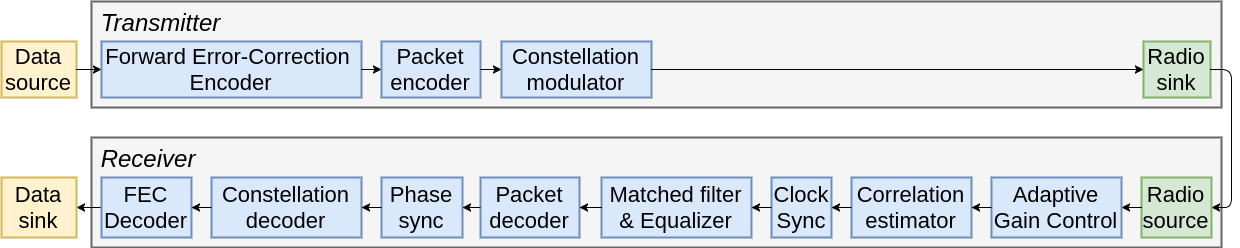
\includegraphics[width=1\textwidth]{img_commchain/overview.png}
    \caption{Communication chain}
    \label{fig:commchain_intro}
\end{figure}

We developed several new blocks to integrate functionality currently not possible in GNU Radio. They will be discussed throughout the report. Extra attention is paid to the packet encoder and decoder in the communication chain. A packet encoder encapsulates the incoming stream into packets, consisting of a preamble, header (containing packet length), payload and checksum. In particular, a flexible packet encoder is implemented, supporting different constellations for preamble, header and payload. The new packet encoder/decoder pair also supports soft-decision error correction and varying packet lengths.\medskip

A small introduction to GNU Radio is provided. The first part of the report focuses on the packet encoder/decoder. The existing packet encoder/decoder pair is evaluated and new, improved blocks are implemented. The second part integrates the new packet encoder/decoder pair in a full-featured wireless communication chain. Problems with the existing frame synchronizer are examined and the improved implementation is discussed. At the end of the report, GNU Radio challenges and limitations are discussed as well as some lessons learned. \medskip

The examples and developed blocks are combined in a GNU Radio module called \textit{packetizer}, located at \url{https://tclgit.epfl.ch/semester-projects/17S-Verelst-GNURadio}.


\section{GNU Radio}


\subsection{Flowgraphs}

GNU Radio implements a dataflow system, where blocks are used to process data. Blocks receive several samples at once in their input buffers, process them and place the result in their output buffer. There are two important ways to pass data from one block to another: streams and message passing.
\paragraph*{Streams}
Streams are the most common way to transmit signal data between blocks. A stream is an endless sequence of samples which have a certain data type. Data types can be distinguished by color, as illustrated in \reff{gnuradio_block}.

\begin{figure}[H]
    \centering
    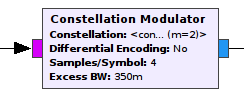
\includegraphics[width=0.3\textwidth]{img_other/gnuradio_block.png}
    \caption{{A GNU Radio block that gets a byte stream as input and outputs complex symbols} }
    \label{fig:gnuradio_block}
\end{figure}

Many data types exist in GNU Radio, but only a few are used in practice. Complex samples are blue, floats are orange and bytes are purple.
\begin{figure}[H]
    \centering
    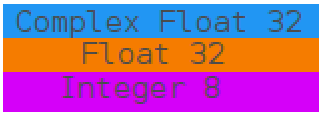
\includegraphics[width=0.25\textwidth]{img_other/datatypes.png}
    \label{fig:datatypes}
\end{figure}

\paragraph*{Tagged streams}
Tagged data streams are an extension of data streams. A tag can be attached to a stream sample, and provides extra control information. Tags are useful to transmit indicators, for example the start and length of a packet.
\begin{figure}[H]
    \centering
    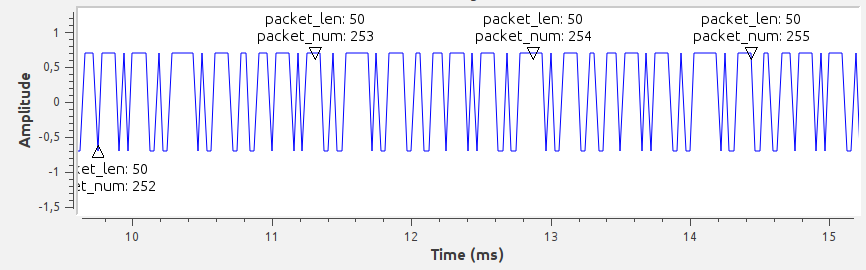
\includegraphics[width=0.95\textwidth]{img_other/tagged_streams.png}
    \caption{Stream tags to indicate the packet start, length and sequence number}
    \label{fig:datatypes}
\end{figure}



\paragraph*{Message passing}
Message passing is a more recent feature, and particularly useful to transmit control and meta data. In contrast to data streams, message passing blocks can be connected to upstream blocks in order to create feedback loops. A message connection is indicated with a dotted line, instead of a solid line.

\subsection{Block development in GNU Radio}
Users can build new Out-of-Tree modules containing new blocks to add extra functionality to the framework.  These blocks are developed in C++ or Python, where C++ focuses on performance and Python on ease of development. A special type of block is a \textit{hier} block, which is a block that internally connects several existing blocks. They can be used to quickly turn existing systems into a separate entity which can be integrated in larger systems.\medskip

We implemented several blocks in this semester project. Technical software development details are not given since block development relies heavily on the GNU Radio API, which can be found online \cite{gr_doxygen}.



\section{Packetization}

\subsection{Current situation in GNU Radio}
\subsubsection{GNU Radio 3.7.9}

Packet encoder and decoder blocks with limited functionality exist in GNU Radio. The \textit{Packet Encoder} and \textit{Packet Decoder} are deprecated blocks that have the following functionality:
\begin{tight_itemize}
\item Create packets with a preamble, acces code, header and a payload. The header is a double repetition of the payload length (16 bits for each field).
\item Constellations: GMSK, DBPSK, DQPSK, D8PSK, QAM8, QAM16, QAM64, QAM256
\item Modulation and pulse shaping with a given number of samples per symbol.
\end{tight_itemize}

The decoder looks for the access code and calculates the number of wrong bits. When this number is under the given threshold, it reads the header to find the payload length. Finally, it outputs the payload as a byte or float stream.

\begin{figure}[H]
    \centering
    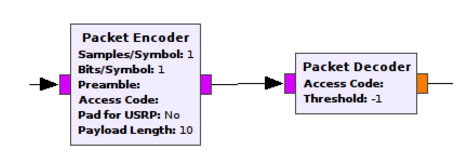
\includegraphics[width=0.6\textwidth]{img_packets/packet_encdec.png}
    \caption{Deprecated packet encoder and decoder blocks}
    \label{fig:packet_encdec}
\end{figure}

The implementation has several limitations:
\begin{tight_itemize}
\item No support for different constellations for preamble, header and payload
\item No proper support for custom header fields. The header is built as a two times the payload length.
\item Lacks flexibility: fixed payload length, pulse shaping not configurable
\item Not enough documentation and the source code is difficult to understand. For example, the output format is not specified.
\end{tight_itemize}

\subsubsection{GNU Radio 3.7.10}
New packet examples are included in this more recent version of GNU Radio. As explained in section 5.2, installing GNU Radio using the recommend way does not guarantee the latest version of GNU Radio. The existence of these packet-related example systems had been discovered late in the project and the project is developed independently.
\newpage
\subsection{Extended Packet Encoder}
\subsubsection{Requirements}
The new packet encoder implementation will limit its functionality to packetizing the incoming data stream with a preamble, header and payload and mapping these to constellation symbols. It will not do any pulse shaping or resampling.\medskip


The new packet encoder supports the following features:
\begin{tight_itemize}
\item GNU Radio's constellation objects in order to support a wide range of PSK and QAM mappings. Optional support for differential encoding.
\item Possibility to use distinct constellation types for preamble, header and payload.
\item GNU Radio's header formatter objects in order to support headers with custom lengths and fields.
\item The start of the payload data for a packet is indicated in the incoming byte stream with a tag that has the payload length as tag value.
\item Optional support for data whitening, as discussed in section 4.4.
\end{tight_itemize}


\begin{table}[H]
  \begin{center}
  \begin{tabular}{|l|l|}

    \hline
    Inputs & Outputs\\
    \hline
    \hline
    Byte stream: 1 bit/byte & Complex: mapped symbols  \\
    A tag should indicate the packet start and length & \\
    \hline

  \end{tabular}
  \end{center}
  \end{table}
   \vspace*{-0.5cm}
  \begin{table}[H]
  \begin{center}
  \begin{tabular}{|l|l|p{6cm}|}
    \hline
    Parameter name & Data type & Description\\
    \hline
    \hline
    Preamble & complex vector & sequence of complex symbols for the preamble\\
    \hline
    Header Constellation & constellation object & pointer to the constellation object for the header\\
    \hline
    Header differential mapping & boolean & use differential encoding for header data\\
     \hline
    Payload Constellation & constellation object & pointer to the constellation object for the payload\\
    \hline
    Payload differential mapping & boolean & use differential encoding for payload data\\
     \hline
    Header Formatter & header formatter object & pointer to the header formatter object\\
     \hline
    Length Tag name & string & name of the tag that indicates the packet start and has the packet length as tag value\\
     \hline
    Zero padding & integer & number of zero symbols (\(0 + 0*j\))  between each packet\\
     \hline
    Whiten & boolean & indicates whether the incoming data stream should be whitened, as discussed in section 4.4.\\
    \hline
  \end{tabular}
  \caption{Interface of the new Extended Packet Encoder block}
  \label{enc_interface}
  \end{center}
\end{table}
 \vspace*{-0.7cm}

\subsubsection{Implementation in GNU Radio Companion}
A prototype system is built in GNU Radio Companion to explore the possibilities of existing blocks. \reff{packets_flowgraph} shows the schematic representation of the dataflow and \reff{packet_encdec} is the GNU Radio implementation with existing blocks. Two main streams can be distinguished:
\begin{itemize}
\item The payload stream is MSB-first repacked to $N$ bits per byte, where $N$ depends on the constellation order. Each of these bytes is mapped to a symbol. More information about MSB-first and LSB-first repacking can be found in appendix \ref{sec:appendix_a}.
\item The header stream is generated by the Packet Header Generator block, which accepts a header formatter object as input. A header formatter object specifies the bit format of the header. The default GNU Radio header for digital transmissions is
the \textit{packet\_header\_default} \cite{packet_header_default_docs} which specifies specifies a 32-bit header as follows:
\begin{tight_itemize}
\item bits 0 - 11: Packet length (LSB first). In this project, the packet length will be defined as the number of payload bits per packet. The maximum payload length value with the default header is $2^{12}-1~=~4095\ bits.$
\item bits 12 - 23: Packet sequence number (auto-incrementing) (LSB first)
\item bits 24 - 31: \gls{crc} for packet header
\end{tight_itemize}

An example illustrates the header format in \reff{pheader}.

\begin{figure}[H]
    \centering
    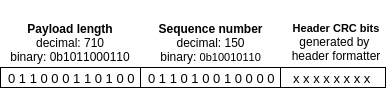
\includegraphics[width=0.6\textwidth]{img_packets/header.png}
    \caption{Example header, for a payload length of 710 bits and a packet sequence number 150. }
    \label{fig:pheader}
\end{figure}




\end{itemize}

The header format is specified in the GNU Radio Companion by adding a variable block with the following value:
\begin{minted}[frame=single,breaklines=true]{C}
digital.packet_header_default(32/constel_header.bits_per_symbol(), "packet_len", "packet_num", constel_header.bits_per_symbol())
\end{minted}
The first argument is the length of the header in symbols. In this example, \textit{constel\_header} is the constellation object that defines the header constellation. The  second argument is the name of the tag carrying the payload length. The third parameter defines which tag name the packet sequence number should get when decoding the header. The last parameter is the number of significant bits per byte at the output. A correct configuration is very important since the Extended Packet Encoder block does not repack the bytes before mapping the header bytes to symbols.
\begin{figure}[H]
    \centering
    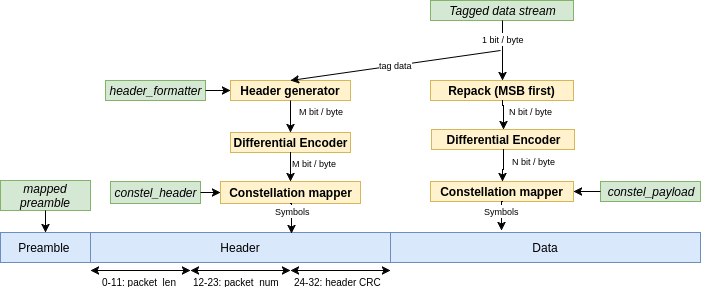
\includegraphics[width=1.05\textwidth]{img_packets/packets_flowgraph_nowhitening_diff.png}
    \caption{Schematic overview of the packet encoder implementation}
    \label{fig:packets_flowgraph}
\end{figure}
\begin{figure}[H]
    \centering
    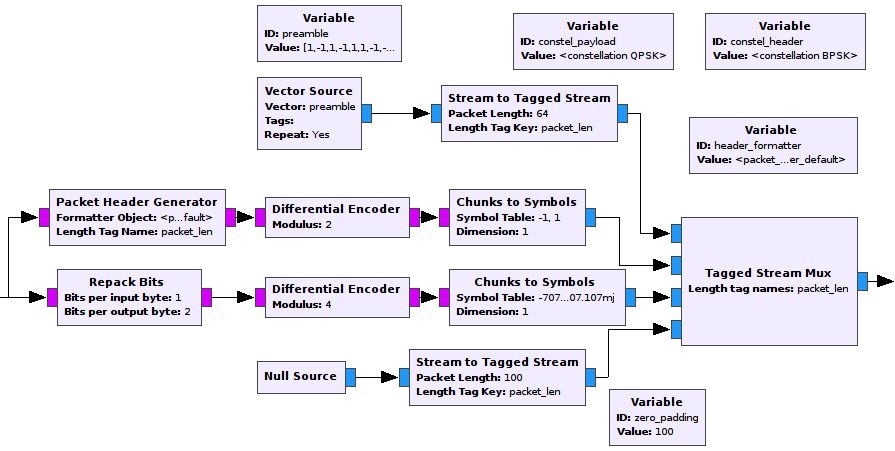
\includegraphics[width=1.05\textwidth]{img_packets/packet_enc_gr2_diff.png}
    \caption{GNU Radio Companion implementation of a packet encoder with differential encoding. Data input on the left has one bit per byte, data output on the right is one complex symbol/sample}
    \label{fig:packet_encdec}
\end{figure}




\subsubsection{Block implementation}
As described in section 2.3, a GNU Radio block can be built in C++ and Python or as a \textit{hier} block that links several existing blocks. In the packet encoder implementation as described above, many blocks do trivial operations that can be efficiently combined to eliminate the overhead of transferring data between blocks. A C++ block is the most appropriate choice.

\begin{figure}[H]
    \centering
    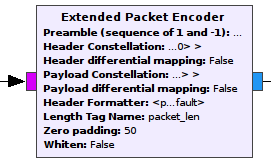
\includegraphics[width=0.45\textwidth]{img_packets/packet_enc_block.png}
    \caption{Extended Packet Encoder in the GNU Radio Companion}
    \label{fig:packet_enc_block}
\end{figure}







\subsubsection{Data example}
A simple test bench is created in order to verify the output of the implemented block. The block processes a predefined data sequence.

\begin{tight_itemize}
\item Preamble (mapped symbols): 1, -1, 1, 1
\item Payload (1 bit/byte): 0,0,0,1,0,0,1,1, \ 1,1,1,1,1,1,1,0, \  1,0,0,0,0,1,1,0, \ 0,0,1,0,1,1,1,1
\item Header mapping: \gls{bpsk} $[0,1] \rightarrow  [1, -1]$
\item Header Formatter: generated by the \textit{packet\_header\_default} class with a length of 32 bits.
\item Payload mapping: \gls{qpsk} \\$[0, 1, 2, 3] \rightarrow[-1-1j, 1-1j, -1+1j, 1+1j]$ 
\end{tight_itemize}

Output:


\begin{minted}[frame=single,breaklines=true]{C}
1,-1,-1,1,
(1+0j), (1+0j), (1+0j), (1+0j), (-1+0j), (1+0j), (1+0j), (1+0j),
(1+0j), (1+0j), (1+0j), (1+0j), (1+0j), (1+0j), (1+0j), (1+0j),
(1+0j), (1+0j), (1+0j), (1+0j), (1+0j), (1+0j), (1+0j), (1+0j),
(1+0j), (-1+0j), (-1+0j), (1+0j), (-1+0j), (-1+0j), (1+0j), (-1+0j), 
(-0.707-0.707j), (0.707-0.707j), (-0.707-0.707j), (0.707+0.707j),
(0.707+0.707j),  (0.707+0.707j), (0.707+0.707j), (-0.707+0.707j), 
(-0.707+0.707j), (-0.707-0.707j), (0.707-0.707j), (-0.707+0.707j), 
(-0.707-0.707j), (-0.707+0.707j), (0.707+0.707j), (0.707+0.707j)) 
\end{minted}

The first 4 symbols are the preamble. The next 32 symbols mapped in \gls{bpsk} have been generated for the header. When demapped to bits, this gives:
\begin{minted}[frame=single,breaklines=true]{C}
00000100 00000000 00000000 01101101
\end{minted}

The payload length in bits is stored in the first 12 bits in an LSB-first way. The decimal result is 32, which is correct. The 12 following bits encode the packet sequence number, 0 in this case. The last 8 bits are a \gls{crc} for the header.
\medskip

The \gls{qpsk} payload symbols demap to:
\begin{minted}[frame=single,breaklines=true]{C}
 00 01 00 11  | 11 11 11 10 | 10 00 01 10 | 00 10 11 11
\end{minted}
Which is the same as the input sequence.










\newpage

\subsection{Extended Packet Decoder}
\subsubsection{Requirements}
The packet decoder does the inverse operation of the packet encoder. It will demap incoming symbols to a data stream. The decoder does not know the packet length, so it should decode the header and retrieve the header length from the corresponding field. \medskip

The Extended Packet Decoder block should support the following functionality:
\begin{tight_itemize}
\item Decoding of packets that are encoded with the Extended Packet Encoder block
\item Support for both hard and soft outputs, in order to support forward error correction
\item Support for differential decoding, when hard-decision decoding is used
\end{tight_itemize}


\begin{table}[H]
\centering
\begin{tabular}{|p{6.5cm}|p{9cm}|}
\hline
 Inputs & Outputs \\ \hline
\multirow{3}{*}{
\pbox{20cm}{Complex: 1 symbol/sample \\ A tag on the incoming stream \\indicates the packet start}} &  Float: soft demapped output, samples between -1 and 1\\ \cline{2-2} 
                  &  Byte: hard demapped output with 1 bit per byte\\ \cline{2-2} 
                  & Message port: message containing header fields \\ \hline
\end{tabular}
\end{table}

\vspace*{-0.5cm}
\begin{table}[H]
\begin{center}
\begin{tabular}{|l|l|p{6cm}|}
\hline
Parameter name & Data type & Description\\
\hline
\hline

Preamble & complex vector & sequence of complex symbols for the preamble\\
\hline
Header Constellation & constellation object & pointer to the constellation object for the header\\
\hline
    Header differential mapping & boolean & use differential decoding for header data\\
\hline
Payload Constellation & constellation object & pointer to the constellation object for the payload\\
\hline
    Payload differential mapping & boolean & use differential decoding for payload data\\
\hline
Header Formatter & header formatter & pointer to the header formatter object for the header\\
\hline
Trigger Tag name & string & name of the tag that indicates the packet start and has the packet length as tag value\\
\hline
Apply Costas Loop & boolean & indicates whether phase synchronization with Costas Loop should be applied.\\
\hline
    Dewhiten & boolean & indicates whether the incoming data stream should be dewhitened.\\
    \hline
\end{tabular}
\caption{Interface of Extended Packet Decoder block}
\label{dec_interface}
\end{center}
\end{table}

\vspace*{-0.7cm}
\newpage
\subsubsection{Implementation in GNU Radio Companion}
A decoder system built in GNU Radio is shown in \reff{packet_decoder_grc}. \reff{packet_decoder_grc_diff} shows a packet decoder with differential decoding. The packet decoder is a complex block that combines several existing solutions:
\begin{tight_itemize}
\item Preamble/Header/Payload Demux: splits the input stream into a header and payload stream. In order to know the payload length, it uses the feedback loop with the decoded header data.
\item Constellation Soft Decoder: demaps symbols to soft bits.
\item Binary Slicer: maps soft bits ($-1$ and $1$) to hard bits ($0$ and $1$).
\item Tagged Stream Fix: drops unnecessary samples so packets are sequential in the stream.
\item Differential Decoder: removes the differential encoding, done in the packet encoder.
\item Packet Header Parser: decodes a header byte stream according to the header format given by the Header Formatter, which is the same one as given to the packet encoder.
\item Costas Loop: applies carrier tracking for phase synchronization, as described in section 4.3.
\end{tight_itemize}



\paragraph*{Preamble/Header/Payload Demux block}
The most important block in the decoder system is the \gls{phpd} block.
It is an extension of the existing Header/Payload Demux block, which is a highly flexible block to extract payload data with a variable length from a packet, by looking at the header fields. The block is implemented as a state machine, and one state had to be added to support preambles. The full state diagram of the \gls{phpd} block is shown in \reff{phpd}. The payload data length is given using the feedback loop for header data. Header data gets decoded and the Packet Header Parser will read the fields from the header. The result is outputted with a GNU Radio message that is forwarded to the \gls{phpd} block.\medskip 

The original Header/Payload Demux block only accepts the payload length as a number of symbols. Since the block does not know the modulation type and order, it can only split the incoming streams into a header symbol stream and payload symbol stream. \medskip

For this project, we added a new parameter called "Header Length value divider". The payload length value, received from the header, will be divided by this number and the result will be ceiled. This modification makes it possible to specify the payload length in bits, while the \gls{phpd} counts symbols.\medskip

For example, when having a payload length of 50 bits and \gls{8psk}, the packet encoder generates one zero-bit to fill all 17 symbols. The packet header carries the value 50 as \textit{packet\_len} field. The \gls{phpd} block is configured with a Header Length value divider of 3, which is the number of bits per symbol. It will calculate $ceil(50/3) = 17$ and output 17 symbols on the payload stream. The first output sample will get a tag with the name \textit{packet\_len} and value 50.\medskip

The Constellation Soft Decoder decodes each symbol to soft bits. In the case of \gls{8psk}, it outputs 3 soft bits per symbol. As a result, the output stream consists of $17\ symbols \times 3\ softbits/symbol = 51\ softbits$ which is not what the \textit{packet\_len} tag indicates. The last bit is a zero bit that is added by the packet encoder to fill the last symbol, and it should be removed from the output. The Tagged Stream Fix block will do this, as explained in the next paragraph \medskip

\begin{figure}[H]
    \centering
    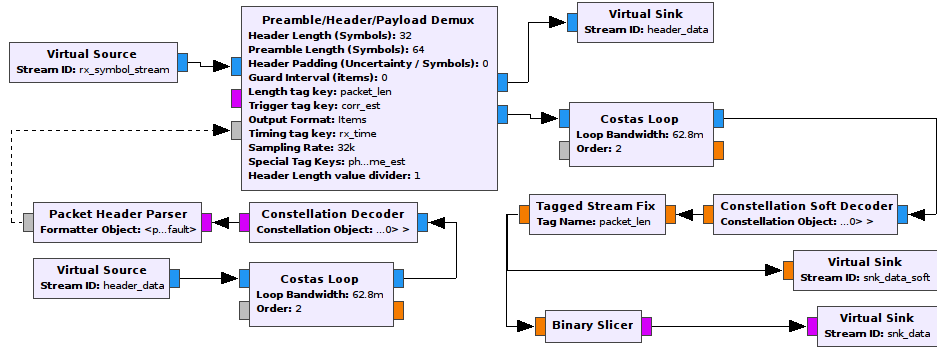
\includegraphics[width=1.05\textwidth]{img_packets/packet_decoder_grc.png}
    \caption{A packet decoder in GNU Radio Companion, configured for a \gls{bpsk} header and \gls{qpsk} payload}
    \label{fig:packet_decoder_grc}
\end{figure}

\begin{figure}[H]
    \centering
    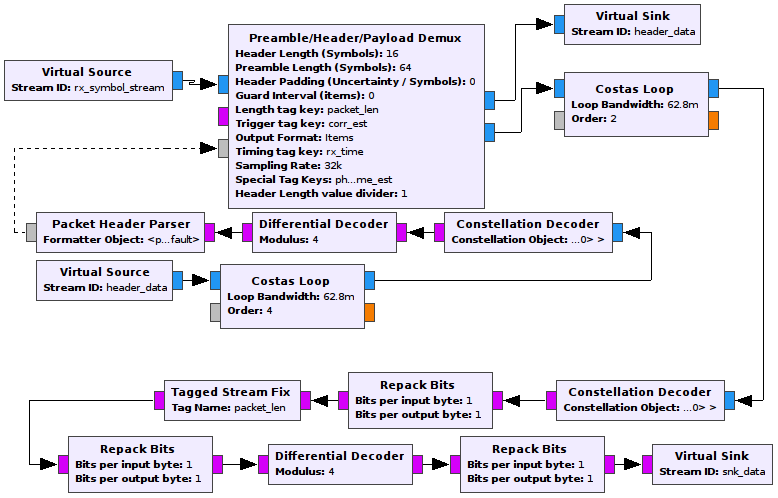
\includegraphics[width=1.0\textwidth]{img_packets/packet_decoder_grc_diff.png}
    \caption{A packet decoder in GNU Radio Companion with differential decoding, configured for a \gls{bpsk} header and \gls{qpsk} payload}
    \label{fig:packet_decoder_grc_diff}
\end{figure}






\begin{figure}[H]
    \centering
    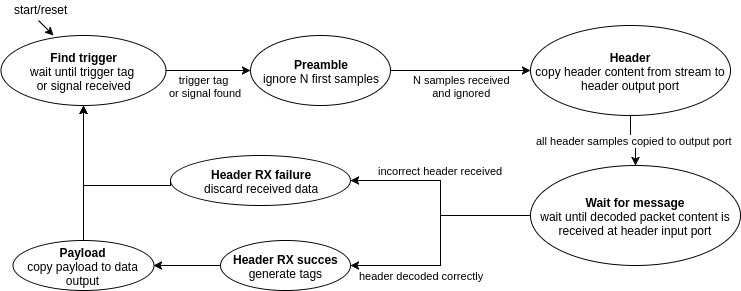
\includegraphics[width=1.05\textwidth]{img_packets/phpd.png}
    \caption{State diagram of the Preamble/Header/Payload block}
    \label{fig:phpd}
\end{figure}

\paragraph*{Tagged Stream Fix block}
A tagged stream with more samples between tags than what the \textit{packet\_len} tag indicates gives problems in GNU Radio's {tagged stream} blocks, such as the Extended Tagged FEC Decoder. These blocks expect that the packets are perfectly sequential, i.e. there are no extra samples between packets. Surprisingly, no GNU Radio block exists to remove the unnecessary samples between packets. \medskip

In this project, a block called \textit{Tagged Stream Fix} has been developed to 'truncate' a tagged data stream. 
It only keeps the samples belonging to a packet, and removes the other samples. This is illustrated in \reff{fixstream}. Because of time constraints during the project, the block is written in Python, even though a C++ block provides more throughput with less CPU usage.
\begin{figure}[H]
    \centering
    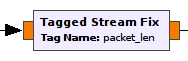
\includegraphics[width=0.3\textwidth]{img_packets/streamfix_block.png}
    \caption{Tagged Stream Fix block in GNU Radio Companion}
    \label{fig:streamfix_block}
\end{figure}
\begin{figure}[H]
    \centering
    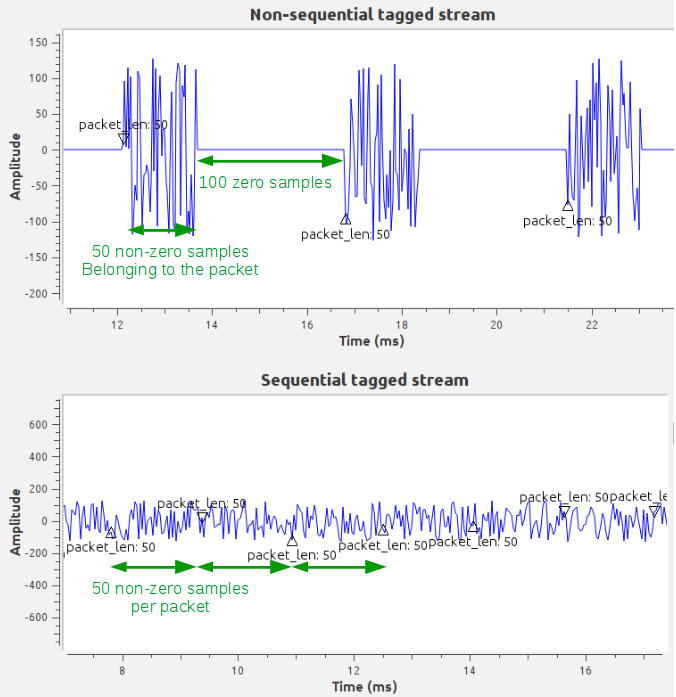
\includegraphics[width=0.9\textwidth]{img_packets/fixstream.png}
    \caption{Illustration of a non-sequential packet stream and a sequential packet stream. In the top plot, the packets are separated with zero samples, in the bottom plot the zero samples are removed.}
    \label{fig:fixstream}
\end{figure}







\subsubsection{Block implementation}
The Extended Packet Decoder block is a combination of several existing blocks, and a \textit{hier} implementation in Python is straightforward. The new block is called Extended Packet Decoder.\medskip

The header data can be analyzed by using the message output port on the Extended Packet Decoder. We developed a new block called Message Sequence Checker  to verify correct packet communication. It reads the $packet\_num$ field from the header and checks for discontinuities in packet sequence numbers. When two the difference between two sequence numbers is more than one, some packets have been dropped because they could not be detected or decoded. The block will output the number of lost packets and the packet loss rate in the console.


\begin{figure}[H]
    \centering
    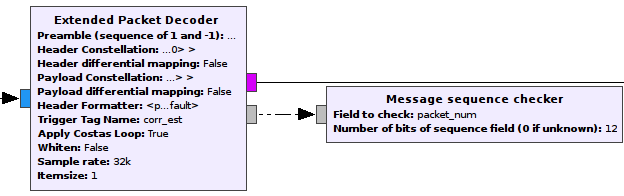
\includegraphics[width=0.8\textwidth]{img_packets/packet_dec_block.png}
    \caption{Extended Packet Encoder block and Message Sequence Checker blocks}
    \label{fig:packet_dec_block}
\end{figure}


\subsection{Packetization example systems}

\subsubsection*{Mapping}
\textit{test\_mapping.grc} is a basic example demonstrating symbol mapping and decoding. Differential encoding/decoding is also implemented.

\subsubsection*{Soft decoding}
\textit{test\_soft\_decoder.grc} illustrates the use of the {Constellation Decoder} block and the {Constellations Soft Decoder} block. An important thing to notice is that the bits should be repacked by MSB-first (instead of the default LSB-first), before mapping the bytes to symbols. The constellation receiver outputs the decoded bits MSB-first.

\subsubsection*{Prototype encoder/decoder}
\textit{encdec\_basic.grc} implements the full-featured packet encoder and decoder using basic GNU Radio blocks. \medskip

\subsubsection*{Packet encoder/decoder blocks }
\textit{encdec\_custom.grc} uses the Extended Packet Encoder/Decoder blocks, with both hard and soft demapping. \medskip
\section{Communication chain}
The communication chain is the set of elements that transforms data into a transmittable waveform. It consists of data pre-processors, modulation units and several recovery units for time, phase and frequency synchronization. An overview of the implemented communication chain is given in \reff{commchain_overview}

\begin{figure}[H]
    \centering
    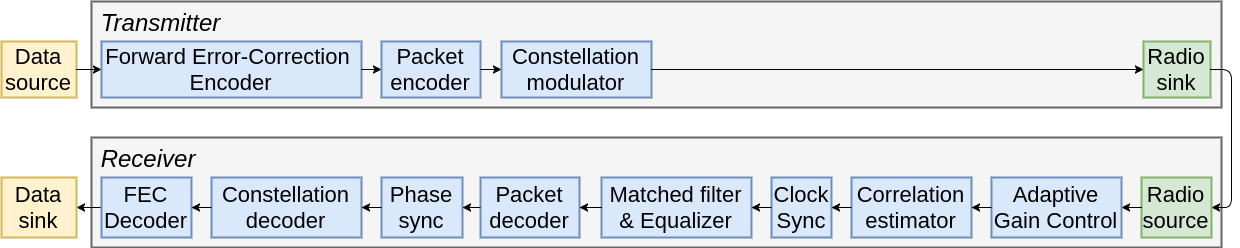
\includegraphics[width=1\textwidth]{img_commchain/overview.png}
    \caption{Communication chain overview}
    \label{fig:commchain_overview}
\end{figure}



\subsection{Pulse shaping}

The implemented packet encoder outputs constellation symbols. These symbols are processed by an upsampler and pulse shaper, in order to limit the bandwidth when transmitting. A common filter is a root raised cosine. At the receiver side, the signal can be convoluted with the matched filter so that the transmission is free of intersymbol interference. The spectrum of a transmissed stream, shaped with a root raised cosine filter, is shown in \reff{channel_spectrum}.

\begin{figure}[H]
    \centering
    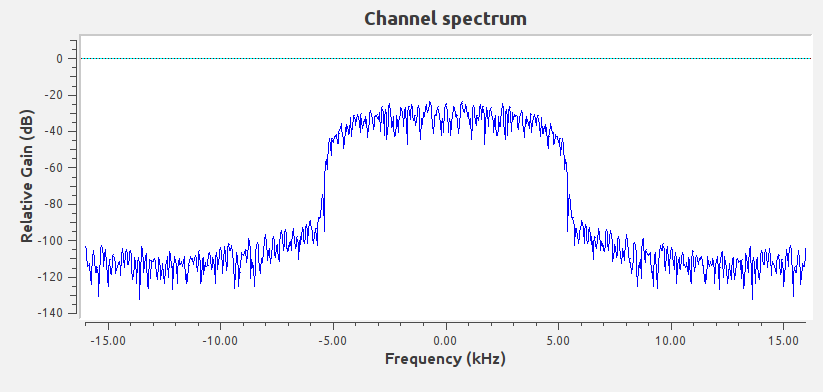
\includegraphics[width=0.8\textwidth]{img_commchain/channel_spectrum.png}
    \caption{Channel spectrum at baseband, RRC-filter with roll-off factor 0.35 and stop-band attenuation of 100 dB}
    \label{fig:channel_spectrum}
\end{figure}




\subsection{Frame synchronization}
The frame synchronization unit detects the start of packets. A common way is to prepend a preamble or access code sequence to the packet content so the receiver side can look for the preamble. After correlating the stream at the receiver with a modulated reference preamble, the packet start can be indicated by detecting correlation peaks.
\subsubsection{GNU Radio situation}
A large number of blocks for synchronization are included in the default GNU Radio installation. The most notable blocks are the \textit{Correlation Estimator}, \textit{Correlate Access Code} and \textit{Correlate and Sync}, where the latter is deprecated since GNU Radio 3.7.10. \medskip


The Correlation Estimator block is the most advanced and updated implementation. The block correlates a given modulated preamble with the incoming stream, and indicates correlation peaks with a tag called \textit{"corr\_est"}. \medskip

The block has a parameter \textit{Tag marking delay} which is used to shift the tag position compared to the incoming data stream. This shifting functionality is required because of two reasons. The first reason is that the convolution, used to pulse shape the reference preamble, introduces extra samples at the beginning and end of the preamble sequence because of the edge effect. When calculating the correlation with the incoming data stream, the tag will be placed at a fixed offset of the real position. The second reason is that some blocks in the communication chain do not preserve the correct tags positions, compared to the samples. The tag delay parameter should be set manually by looking at the output scopes.\medskip

\begin{figure}[H]
    \centering
    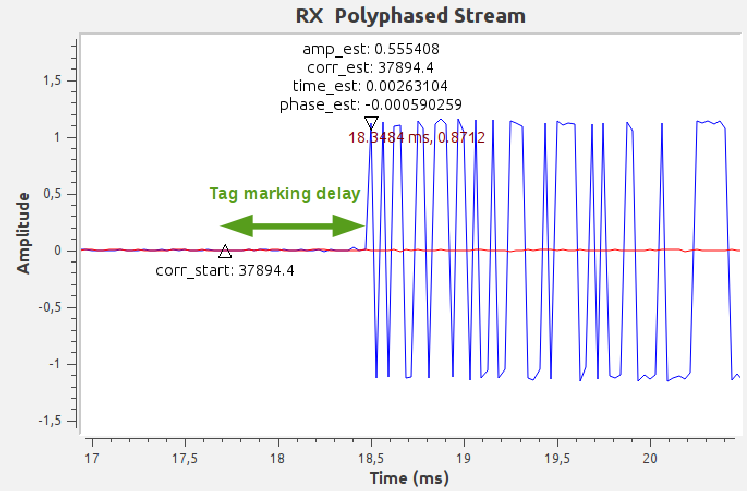
\includegraphics[width=0.8\textwidth]{img_commchain/tag_marking_delay2.png}
    \caption{The \textit{corr\_start} tag indicates where the Correlation Estimator block detected the preamble. The other tags are shifted by the number of samples that is given in the Tag Marking Delay field.}
    \label{fig:tag_marking_delay2}
\end{figure}

The $gr$-$digital$ package includes several synchronization examples, which are unfortunately broken in GNU Radio 3.7.9 and 3.7.10. The \textit{test\_corr\_est.grc} example has a threshold that is far too small, which causes a large amount of false-positives. In addition, the "Tag marking delay" is wrong. Many GNU Radio users have reported these issues \cite{corr_est_github_issue}.





\subsubsection{Pulse shaping the reference preamble}
The Correlation Estimator block expects a modulated and shaped preamble as input argument. \medskip

GNU Radio has a complementary block to modulate and pulse shape a byte stream, called Modulate Vector. In this project however, the preamble is defined as a pre-mapped sequence of complex symbols. To pulse shape the mapped vector, a new block was implemented in Python. The block is called Pulse Shape Vector and will pulse shape a given vector with a given filter. \medskip

\begin{figure}[H]
    \centering
    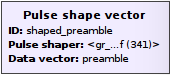
\includegraphics[width=0.25\textwidth]{img_commchain/pulseshaper_block.png}
    \caption{Pulse Shape Vector block in GNU Radio Companion}
    \label{fig:pulseshaper_block}
\end{figure}

The block accepts three parameters: 
\begin{tight_itemize}
\item ID: the variable name for the shaped preamble (output of the block)
\item Data vector: the variable name of the mapped preamble
\item Pulse shaper: definition of a filter in GNU Radio.
When using a polyphase filterbank with root raised cosine taps, the filter is defined is as follows:
\begin{minted}[frame=single,breaklines=true]{C}
filter.pfb_arb_resampler_ccf(
 sps,
 firdes.root_raised_cosine(nfilts, nfilts, 1.0, eb, 11*sps*nfilts),
 32
) 
\end{minted}
The meaning of the arguments can be found in the GNU Radio manual for the polyphase filterbank \cite{gr_pfb} and root raised cosine \cite{gr_rrc}.
\end{tight_itemize}




\subsubsection{Problems with the Correlation Estimator block}
The existing correlation estimator implementation was not sufficient to achieve a reliable packet detection. Three problems were identified:
\begin{enumerate}
\item The threshold cannot be set high enough to avoid false detections when having a high input power. When the threshold is set to 0.99999998 or higher, the system execution stops without returning any error.
\item False detections occur when there is no incoming signal except noise. 
\item Especially at the end of a packet, several false detections occur even when having a high signal power.
\end{enumerate}
These problems are illustrated in \reff{corr_est_false2}.

\begin{figure}[H]
    \centering
    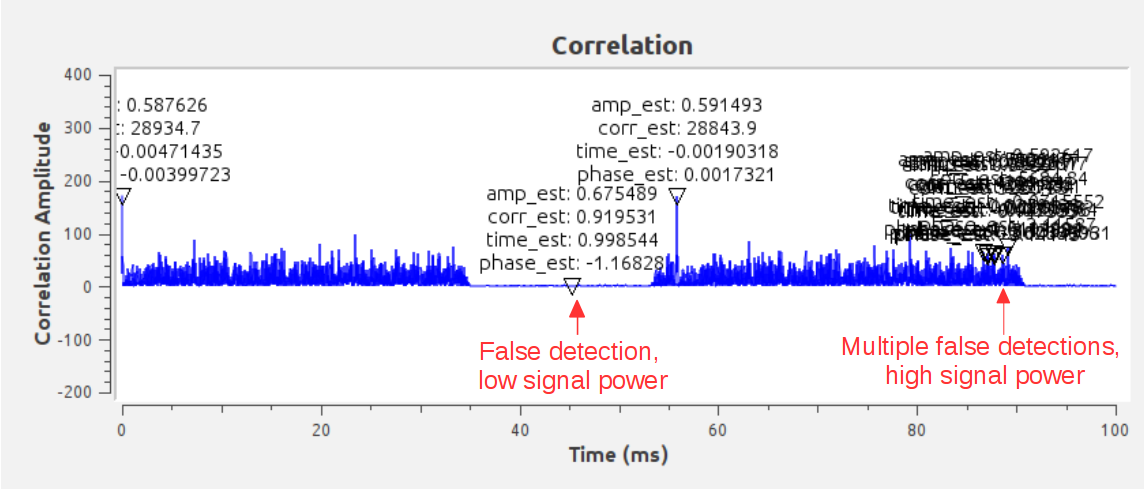
\includegraphics[width=0.8\textwidth]{img_commchain/corr_est_false2.png}
    \caption{Correlation Estimator false detections}
    \label{fig:corr_est_false2}
\end{figure}




\paragraph*{Internal working of the existing implementation }

In order to detect a correlation peak, the incoming signal is correlated with the modulated reference preamble. The squared magnitude of each correlation sample is calculated and if the squared correlation magnitude of a sample is larger than the \textit{detection threshold}, the sample is marked with a tag. Since the correlation magnitude depends on the incoming signal level, adaptive gain control should be used to normalize the signal power.\medskip

The detection method can be expressed in formulas as follows. \textit{Incoming\_signal} is the incoming symbol sequence of length $N$ and \textit{mod\_preamble} is the modulated preamble symbol sequence. The exact way to determine the \textit{detection\_threshold} is explained in the next paragraph.  

\setlength{\abovedisplayskip}{1pt}
\setlength{\belowdisplayskip}{1pt}
\begin{align*}
 corr = correlate(incoming\_signal, mod\_preamble)
\end{align*}
\begin{align*}
 corr\_mag\_sq[i] = corr[i]^2 \quad \forall i = 0\ to\ N-1
\end{align*}
\begin{align*}
detection[i] = corr\_mag\_sq[i] > detection\_threshold \quad \forall  i = 0\ to\ N-1
\end{align*}
\smallskip

Up to GNU Radio 3.7.9, the Correlation Estimator block used a fixed detection threshold. The \textit{detection\_threshold} value is relative to the power of the discrete autocorrelation of the modulated reference preamble.  The value is constant and does not depend on the incoming signal. The parameter $threshold$ can be defined by the user:

\begin{align*}
preamble\_autocorr =  \sum_{i}{|mod\_preamble[i] * mod\_preamble[i]^*|}
\end{align*}
\begin{align*}
detection\_threshold = threshold * preamble\_autocorr^2;
\end{align*}
\smallskip




In GNU Radio 3.7.10, the fixed detection threshold was changed to an adaptive threshold, to avoid the need for adaptive gain control. That implementation uses a constant false alarm rate (CFAR) detection method. The given \textit{threshold} parameter is converted to a probability of false alarm (pfa):

\begin{align*}
 d\_pfa = -\log (1- threshold)
\end{align*}
\smallskip

The final detection level is a multiplication of the average correlation magnitude of surrounding samples and the probability of false alarm:

\begin{align*}
 detection\_threshold = 4 * d\_pfa * mean(corr\_mag\_sq\ of\ surrounding\ samples)
\end{align*}
\smallskip

The decision algorithm is also slightly modified. A sample is indicated as a packet start if the sum of the squared correlation magnitude of this sample \textit{i} and the next sample \textit{i+1} is greater than the detection threshold. The sum is introduced to counter the effect of a time offset, which can spread the correlation peak over two samples.

\begin{align*}
	detection = (corr\_mag[i] + corr\_mag[i+1]) > detection\_threshold
\end{align*}
\smallskip


\subsubsection{Improved Correlation Estimator}
We modified the Correlation Estimator, and included a new block called Correlation Estimator 2 in the \textit{packetizer} module. This new block solves the problems described in the previous section, by doing several modifications in the C++ code.

\paragraph*{Solving problem 1: Increasing the maximum threshold}

The internal representation of the $threshold$ parameter variable is a float. The limited precision of a float causes numerical problems when calculating \( d\_pfa = -\log (1- threshold)\). In fact, the closest float to 1 is 0.999999880791. Anything closer to 1 will be rounded to 1 and that gives the logarithm of 0, which is impossible to compute. \medskip

By changing the internal threshold representation from float to double, a much larger threshold can be chosen.

\paragraph*{Solving problem 2: False detections when no signal}
Detecting a packet when the incoming signal level is very low is not useful, since the SNR will probably be too low to decode the packet. By adding a fixed threshold in parallel to the adaptive threshold, a minimum signal power can be set. The fixed threshold is implemented in the same way as the one in Correlation Estimator block in GNU Radio 3.7.9, by setting the minimum ratio between the correlation magnitude and autocorrelation value of the preamble.

\paragraph*{Solving problem 3: False detections at the end of the packet}

The adaptive threshold sets the detection threshold based on the mean squared magnitude of surrounding samples. The Correlation Estimator block averages all the samples that are currently being processed in the block. The amount of samples that is passed between blocks in the dataflow graph is chosen by the GNU Radio scheduler, and can change during execution.  %TODO
\reff{corr_dataflow} visualizes  which samples were considered when averaging the correlation values at a particular instant. The \textit{START} tag indicates the first sample of a dataflow sample group, and all subsequent samples up to the next \textit{START} tag are processed at once in the block.\medskip

It is clear that this way is not optimal when only a part of the sample group has a significant amplitude. In that case, the threshold will be low and false positives occur on the few samples with significant amplitude.\medskip

The problem can be solved by defining a fixed number of samples to average. In the improved implementation of the Correlation Estimator block, the amount of samples is based on the amount of samples of the modulated reference preamble. For a BPSK preamble of 64 symbols shaped with 4 symbols per sample, the Correlation Estimator will average $256/2$ samples to set the detection threshold. These samples are chosen around the sample of interest, i.e. the sample that is currently being checked.\medskip

\begin{figure}[H]
    \centering
    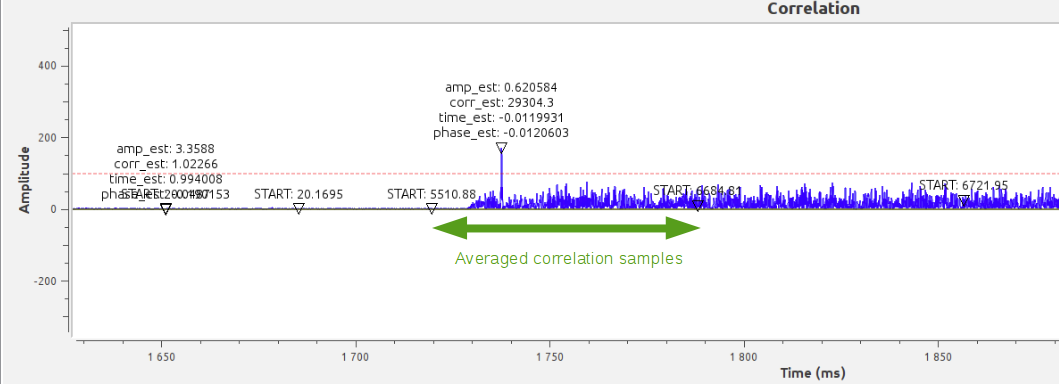
\includegraphics[width=1\textwidth]{img_commchain/corr_dataflow.png}
    \caption{{Correlation samples}}
    \label{fig:corr_dataflow}
\end{figure}

\paragraph*{Block in GNU Radio Companion}
The Correlation Estimator 2 block is also included in the new $gr$-$packetizer$ package made for this project. The block is shown in \reff{corr_est_2}. The block has two extra parameters compared to the original Correlation Estimator block: \textit{Fixed threshold} and \textit{Verbose}.
\begin{tight_itemize}
\item Symbols: symbols of the modulated and pulse shaped preamble
\item Samples per Symbol: upsampling factor 
\item Tag marking delay: tag position delay (number of samples) compared to detection instant
\item Threshold: threshold value to set the \textit{probability of false alarm} variable for the adaptive threshold
\item Fixed threshold: threshold value to set the fixed threshold, which is relative to the power of the autocorrelation
\item Verbose: output a message in the console when a peak has been detected, with the peak value, the current adaptive threshold value and the fixed detection thresholds
\end{tight_itemize}


\begin{figure}[H]
    \centering
    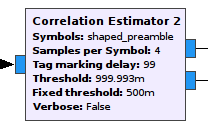
\includegraphics[width=0.35\textwidth]{img_commchain/corr_est_2.png}
    \caption{{Correlation Estimator 2}}
    \label{fig:corr_est_2}
\end{figure}

\subsection{Time and phase synchronization} \label{section_time_phase_sync}
The Correlation Estimator can derive time and phase information by looking at the correlation result. The block will communicate this information by adding the tags \textit{phase\_est} and \textit{time\_est} to the stream.\medskip

The Polyphase Clock Sync block is a time synchronizer that is compatible with the \textit{time\_est} tag. Its purpose is to realign and downsample the incoming stream so the signal samples of the output signal are sampled at exactly the peak of the sinc shape introduced by the root raised cosine filter. The block immediately applies the matched pulse shaping filter using a polyphase filter bank, so the block outputs constellations symbols.\medskip

Costas Loop is a phase synchronizer that optionally uses the \textit{phase\_est} tag. In fact, Costas Loop uses a phase-locked loop to track the carrier frequency. \reff{costas_phase} shows the effect of Costas Loop when a fixed phase offset is seen by the receiver. \reff{costas_freq} illustrates the case where a carrier frequency offset has been applied. Costas Loop will lock to the carrier frequency and align constellations to their correct positions. The \textit{phase\_est} tag helps to quickly correct the phase by indicating the estimated phase offset.\medskip

GNU Radio's Costas Loop expects the modulation order as an input parameter. The modulation order for phase-shift keying modulations is \(2^{N}\), where $N$ is the number of bits per symbol. Costas Loop in GNU Radio is limited to the modulation orders 2 (\gls{bpsk}), 4 (\gls{qpsk}) and 8 (\gls{8psk}). \medskip

The packet encoder/decoder pair implemented in this project supports different constellation types for preamble, header and payload. This implies that the Costas Loop block can only be applied after the header and payload have been split by the Preamble/Header/Payload Demux block. The header decoder stream and payload decoder stream have their own phase synchronizers that receive bursts of header or payload data, as shown in \reff{packet_decoder_grc}. The phase can have large discontinuities between those bursts, which makes it more difficult for the phase-locked loop to lock to the carrier and reduces the performance of Costas Loop. \medskip


\begin{figure}[H]
    \centering
    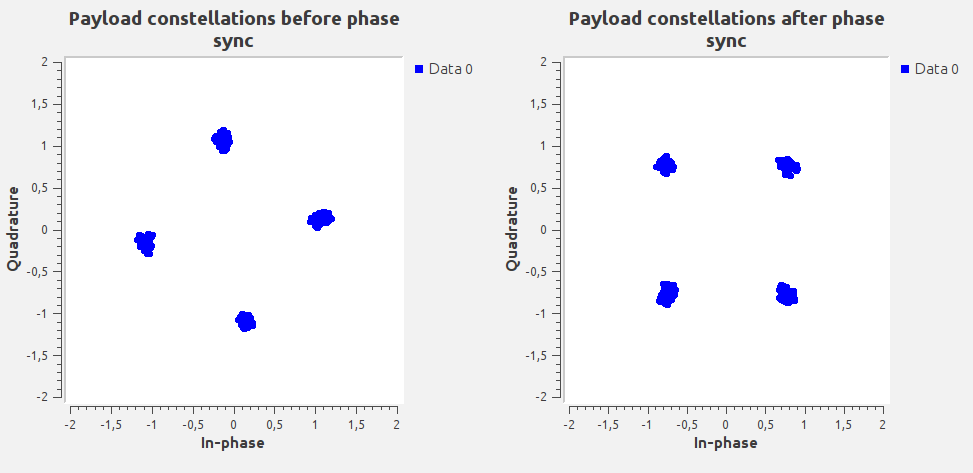
\includegraphics[width=0.8\textwidth]{img_commchain/phase_sync.png}
    \caption{Effect of Costas Loop when receiving constellations with a fixed phase offset }
    \label{fig:costas_phase}
\end{figure}



\begin{figure}[H]
    \centering
    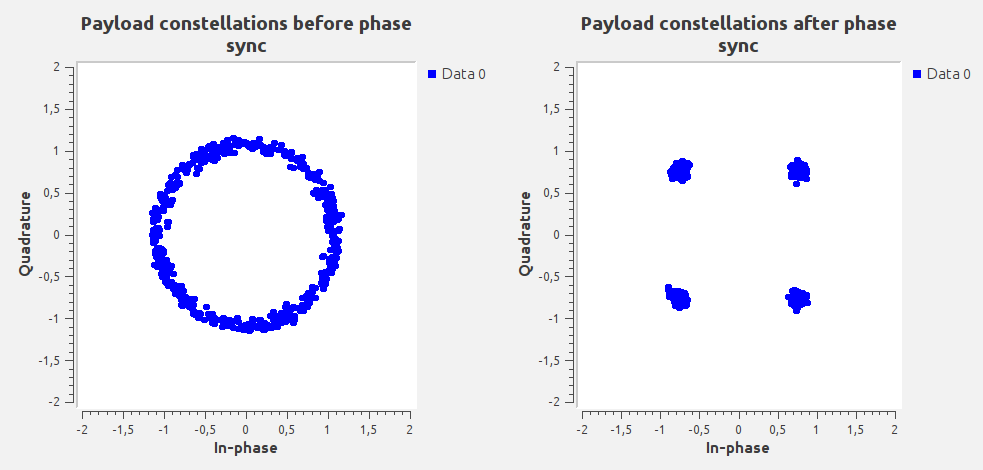
\includegraphics[width=0.8\textwidth]{img_commchain/phase_sync2.png}
    \caption{Effect of Costas Loop as a frequency tracker}
    \label{fig:costas_freq}
\end{figure}

\subsubsection{Test systems}
\textit{test\_time\_phase\_sync.grc} is an extension of mapping example \textit{test\_mapping.grc}. The symbols are shaped with a root raised cosine filter. A channel model is added to simulate a time offset, frequency offset, phase offset and noise in the signal. Time and phase synchronization is added with the Polyphase Clock Sync block and Costas Loop. A BER output is also provided, which can be used to analyze the effects of the channel. It is used to verify the correct working of the communication chain.





\subsection{Data whitening}

Data grouped in packets can contain long sequences of 0's and 1's. The lack of signal variation can be problematic for adaptive circuits such as adaptive gain control and phase-locked loops.\medskip

Data whitening or scrambling is a technique to eliminate long sequences of 0's and 1's. A simple additive synchronous whitener is implemented in this project, which whitens incoming data bytes by applying $XOR$ operations with a pseudo-random sequence. Data can be dewhitened by applying the same $XOR$ operations. The implementation is synchronous because the pseudo-random sequence needs to be reset to align with the data stream. Since this project uses packet-based communications, synchronization is straightforward: at the start of a packet, the random sequence is reset.\medskip

The whitener implementation is split in a kernel and a block interface. The kernel is a general implementation which can be used as a standalone whitener. The packet encoder uses this kernel to whiten incoming data. The kernel is in fact both a whitener and dewhitener, since the inverse operation of an $XOR$ is itself.\medskip

The block interface wraps the kernel in a standalone GNU Radio block. It manages the input and output of items and provides an interface to configure the block. The whitener block then initializes the whitener kernel depending on the given arguments.

\subsubsection{Whitener kernel}
The whitener kernel is a C++ class that performs the whitening operations. The class $gr/packetizer/kernel/whitener.h$ defines three constructors:
\begin{enumerate}
\item $whitener();$\\
Initializes a whitener object for 8 significant bits per byte using a linear-feedback shift register.

\item $whitener(int\ bits\_per\_byte);$\\
Initializes a whitener object for $bits\_per\_byte$ significant bits per byte using a linear-feedback shift register.

\item $whitener(std::vector<unsigned\ char> random\_mask, int\ bits\_per\_byte);$\\
Initializes a whitener object for $bits\_per\_byte$ significant bits per byte using the given $random\_mask$ to XOR data with. If $random\_mask$ is an empty vector, a pre-computed random mask will be used.
\end{enumerate}

After initialization, the whitener object can be used to process data by executing its method:

\begin{minted}[frame=single,breaklines=true]{C}
/*!
* Do the whitening. Starts reading data in at pointer data_in
* Starts outputting data at data_out
* Processes data_length bytes of data.
*/
void
do_whitening(const unsigned char* data_in, unsigned char* data_out, unsigned int data_length, unsigned int whitening_offset);
\end{minted}

\subsubsection{Whitener block}

The whitener block is called the Tagged Stream Whitener. A \textit{tagged stream} in GNU Radio expects a stream where data is combined in packets with a tag indicating the packet start and length. The block is both a whitener and dewhitener. After whitening, the original data can be recovered by applying the same block with the same parameters on the whitened stream.

\begin{figure}[H]
    \centering
    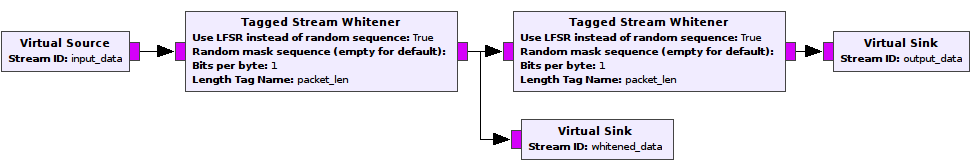
\includegraphics[width=1\textwidth]{img_commchain/whitener_chain.png}
    \caption{The Tagged Stream Whitener in GNU Radio Companion. The left block whitens the data and the right one dewhitens data.}
    \label{fig:whitener_data}
\end{figure}


\subsubsection{Test system}
\textit{test\_whitener.grc} illustrates the use of the \textit{Tagged Stream Whitener} blocks.



\begin{figure}[H]
    \centering
    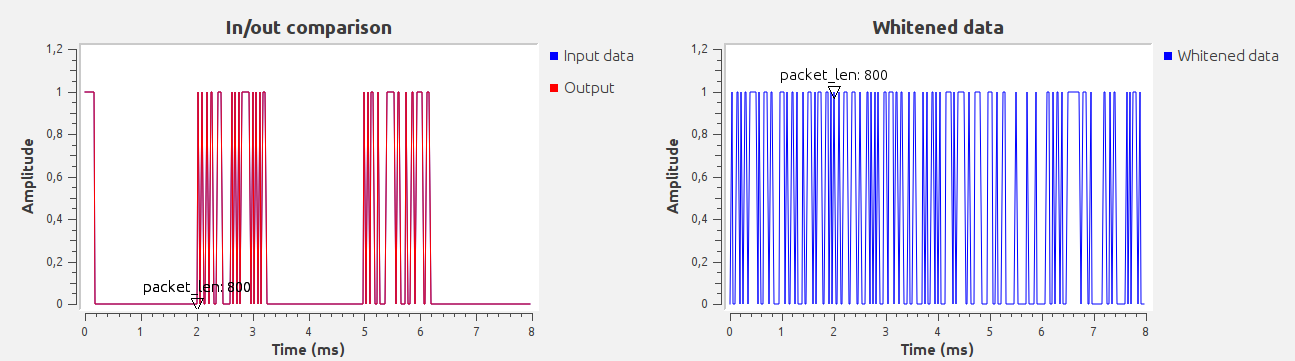
\includegraphics[width=1\textwidth]{img_commchain/whitener.png}
    \caption{Non-whitened data on the left has long sequences of 0 bits. }
    \label{fig:whitener_data}
\end{figure}

\begin{figure}[H]
    \centering
    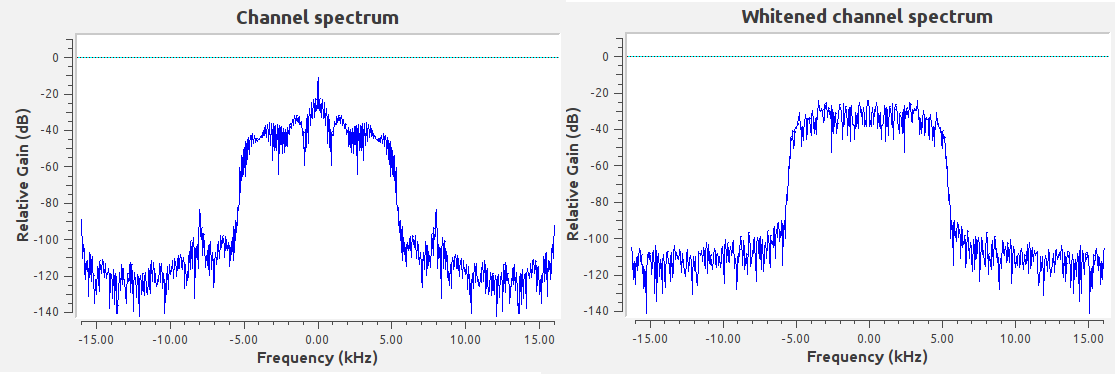
\includegraphics[width=1\textwidth]{img_commchain/whitened_spectrum.png}
    \caption{The non-whitened spectrum is unbalanced and has a DC peak. }
    \label{fig:whitener_spectrum}
\end{figure}




\subsection{Forward Error Correction}

\gls{fec} or channel coding pre-processes the data by adding redundancy to make communications more reliable in noisy channels. Encoding data in a redundant way is done with an error-correcting code.  \medskip

GNU Radio has a dedicated package with \gls{fec} modules called $gr$-$fec$ which is extensively documented. \cite{gr_fec_docs} % REF https://gnuradio.org/doc/doxygen/page_fec.html
The \gls{fec} API is split on two levels: variables and deployments. A variable implements error-correcting code in encoding and decoding methods. A deployment is the connection between the flowgraph and the variable. It will handle the setup and data passing between blocks. \medskip

Several error-correcting codes are defined. A standard convolutional coder is used in this project in combination with the FEC Extended Tagged Encoder and FEC Extended Tagged Decoder as deployments. The \gls{fec} encoder is placed right before the packet encoder, and the \gls{fec} decoder right after the packet decoder. The FEC Extended Tagged Decoder has a float input and can use soft-decision decoding. 



\subsubsection{Test systems}
\textit{test\_fec.grc} illustrates the use of the \textit{FEC Extended Tagged Encoder} and \textit{FEC Extended Tagged Decoder}. Note that the FEC encoder expects a data stream of bytes with 1 significant bit per byte. The output of the encoder is manually mapped to soft bits (-1 and 1). A separate CC Decoder object is set for each FEC decoder.\medskip

\textit{encdec\_custom\_fec.grc} implements a packet encoder and decoder combined with forward error correction,  with hard and soft decisions.



\subsection{Communication chain example systems}
\subsubsection*{Communication chain with Extended Packet Encoder/Decoder blocks}
\textit{chain\_custom.grc} implements the full communication chain with packet encoder, pulse shaper, channel modeler, adaptive gain control, correlation estimator (preamble detector), time synchronization and the packet decoder (which includes phase synchronization).

\subsubsection*{Communication chain with RX receiver built with fundamental blocks}
\textit{chain\_rx\_debug.grc} implements the same communication chain as the previous example. In this example, the packet decoder is built using separate blocks, in order to debug the individual components of the packet decoder. This example can also be used to implement extensions of the packet decoder.

\subsubsection*{Communication chain with RX receiver built with fundamental blocks}
\textit{chain\_rx\_debug\_differential.grc} is the same as \textit{chain\_rx\_debug.grc}, but with differential decoding.


%\section{Example circuits}
This section describes the example circuits to test implemented blocks. The files are located in the $Examples$ folder in the Out-of-Tree module $gr$-$packetizer$

\subsection{Basic test circuits}

\subsubsection*{Mapping}
\textit{test\_mapping.grc} is a basic example demonstrating mapping by using the \textit{Chunks to Symbols} block and decoding with the \textit{Constellation Decoder}.

\subsubsection*{Time and phase synchronization}
\textit{test\_time\_phase\_sync.grc} is an extension of mapping example. The symbols are shaped with a root raised cosine filter. A channel model is added to add a time offset, frequency offset, phase offset and noise to the signal. Time and phase synchronization is added with the Polyphase Clock Sync block and Costas Loop. A BER output is also provided to analyze the effects.


\subsubsection*{Soft decoding}
\textit{test\_soft\_decoder.grc} illustrates the use of the {Constellation Decoder} block versus the {Constellations Soft Decoder} block. An important thing to notice is that the bits should be repacked by MSB first (instead of the default LSB first), before mapping the bytes to symbols. The constellation receiver seems to output the decoded bits MSB-first.

\subsubsection*{Forward Error Correction}
\textit{test\_fec.grc} illustrates the use of the \textit{FEC Extended Tagged Encoder} and \textit{FEC Extended Tagged Decoder}. Note that the FEC Encoder expects a data stream of bytes with 1 significant bit per byte. The output of the encoder is manually mapped to soft bits (-1 and 1). \medskip

\textit{test\_fec\_soft.grc} illustrates the combination of FEC and constellations encoding/decoding. Note that a CC Decoder object has been set for each FEC Decoder.

\subsubsection*{Whitener}
\textit{test\_whitener.grc} illustrates the use of the \textit{Tagged Stream Whitener} blocks.











\subsection{Packet encoder/decoder}
\subsubsection*{Basic encoder/decoder}
\textit{encdec\_basic.grc} implements the full-featured packet encoder and decoder using basic GNU Radio blocks. Note that his examples crashes after about 490 generated packets. This is due to a scheduling problem with the packet encoder part. \medskip

%\subsubsection{Basic encoder/decoder with FEC}
\textit{encdec\_basic\_fec.grc} implements a packet encoder and decoder combined with forward error correction, both with hard and soft demapping. Again, this example crashes after a few seconds.


\subsubsection*{Packet encoder/decoder blocks }
\textit{encdec\_custom.grc} uses the extended packet encoder/decoder blocks, for both hard and soft demapping. \medskip


%\subsubsection{Packet encoder/decoder blocks with FEC}
\textit{encdec\_custom\_fec.grc} uses the extended packet encoder/decoder blocks, for both hard and soft demapping in combination with forward error correction. Note that only the FEC Decoder that uses the soft output produces completely correct results. When using hard decoding, some decoding mistakes occur, even though the output data of the soft and hard demapper is exactly the same.

\subsection{Communication chain}
\subsection*{Communication chain with extended packet encoder/decoder blocks}
\textit{chain\_custom.grc} implements the full communication chain with packet encoder, pulse shaper, channel modeler, carrier tracking, adaptive gain control, correlation estimator (preamble detector), time synchronization and the packet decoder (which includes phase synchronization).

\subsubsection*{Communication chain with RX receiver built with fundamental blocks}
\textit{chain\_rx\_debug.grc} implements the same communication chain as the previous example, except the carrier tracking. In this example, the packet decoder is built in fundamental blocks, in order to debug the individual components of the packet decoder.










\section{GNU Radio Challenges, Shortcomings and Lessons Learned }


\subsection{Existing blocks}
GNU Radio is open-source software and constantly in development. Blocks can behave inconsistently because they are mostly contributed by enthusiasts. For example, some blocks do not process tags well because the tagging system was introduced later. In addition, extensive documentation and examples are often lacking or they are outdated. \medskip


GNU Radio has a steep learning curve, and it can be challenging to get an overview of all possibilities and features. In general, knowledge of GNU Radio API's and block development is very useful when implementing a system. Often it is only possible to get the desired functionality with a custom implementation. The knowledge of GNU Radio development is also useful when evaluating existing blocks.\medskip

Several blocks have similar functionality. For example, blocks related to frame synchronization are: $Correlation\ Estimator$, $PN\ Correlator$, $Correlate\ and\ Sync$, $Simple\ Correlator$, $Correlate\ Access\ Code\ \-\ Tag\ Stream$, $Correlate\ Access\ Code\ -\ Tag$. % TODO Fix the misuse of latex code tags 
Some of these blocks are undocumented, some have no examples and some of them do not work at all with the latest version of the framework. \medskip

Blocks used for repacking bytes also demonstrate this, as \textit{Pack K bits}, \textit{Unpack K bits}, \textit{Packed to Unpacked} and \textit{Unpacked to Packed} do not propagate tags. The best implementation is the \textit{Repack Bits} block which works for both repacking and unpacking, and propagates tags.\medskip

Often, parameters should be set by guessing an initial value and looking at the effect. Phase locked loops have  a loop bandwidth parameter which is not well defined and documentation says it should be set around $2*pi/100$. \medskip


\subsection{Installing GNU Radio}

Even the installation of GNU Radio can be challenging for a beginner. Although binaries for Windows exist, it is strongly recommended to use GNU Radio in Linux, especially when developing Out-of-Tree modules. Many dependencies and libraries are tedious to install under Windows. \medskip

This project was made on Ubuntu, and one has to be careful when installing GNU Radio. The recommended way % TODO REF https://wiki.gnuradio.org/index.php/InstallingGR
to install GNU Radio is via the gnuradio package from your distribution's standard repositories \cite{gr_install}. On Ubuntu 16.04, these binaries install the older GNU Radio 3.7.9. In order to get the most recent version, GNU Radio should be built from source.\medskip

When installing from source, some optional dependencies might not be available, and GNU Radio will not explicitly notify this. During this project, the FEC Decoder block returned a debug message for every decoded packet. When transmitting at high throughput, the continuous flow of debug messages in the console made the GNU Radio Companion crash.\medskip

This behavior is caused by the lack of the \textit{log4cpp} dependency. Although several ways to disable debug messages are proposed on the internet \cite{gr_logging} , the only short-term way that helped in this project was rebuilding GNU Radio with a parameter: % TODO source 
\begin{minted}[frame=single,breaklines=true]{C}
cmake -DENABLE_GR_LOG=off <srcdir>
\end{minted}
This solution is inconvenient and will also disable all other debug messages, except fatal errors.

\subsection{Debug possibilities}
Debugging input/output data is rather difficult in GNU Radio, especially when implementing a system in GNU Radio Companion. The common way to view signals is to attach a scope as output, but there is no convenient way to pause a system, to analyze the current state. A workaround is to add a slider to the GUI which controls the sample rate. While a sample rate of 0 does not have the desired effect, a sample rate of 1 does freeze the system. The tag positions are not always correctly displayed in the GUI plots when decreasing the sample rate to very low values. \medskip

Systems lock up when the scheduler cannot balance the data flow in the system. This may happen when a block, that has two ports which consume the same amount of samples per time instant, receives data streams with a different number of samples per second. GNU Radio will not indicate the block that is causing problems. \medskip

In general, it is challenging for beginners to locate the problem when something is not working. It could be the wrong use of an undocumented block, a wrong parameter or a problem with the block's implementation.

\subsection{Block development}
Block development uses the GNU Make to compile the code and install the blocks. GNU Radio provides an excellent beginner tutorial to learn coding blocks in both C++ and Python. The amount of tools and interfaces can be overwhelming. The \textit{gr\_modtool} facilitates the development of GNU Radio blocks by auto-generating the required config files, but sometimes minor adjustments have to be made manually.
\begin{tight_itemize}
\item Make: terminal commands, makelists
\item SWIG: interface files
\item GNU Radio development: several APIs for blocks and data transfer
\item GRC: XML with Cheetah templates as an interface between Python and GRC
\end{tight_itemize}
Often, the trial-and-error involved in the process can be cumbersome. For example, the process when installing an Out-of-Order module consists of the following terminal commands:
\begin{minted}[frame=single,breaklines=true]{C}
cd /path/to/oot/module
mkdir build
cd build
cmake ../
make
sudo make install
sudo ldconfig
\end{minted}
When changing the block's main initializer in a C++ header file, these steps will not work if the project was already compiled before.  SWIG will throw an error mentioning the arguments in the header file are not correct. Beginners might think there is a problem with the C++ code, but in fact, the \textit{build} folder has to be removed in order to remove the old compiled files and caches.

\section{Conclusion}
The main goal of this project was to become familiar with GNU Radio and implement a communication chain with an improved packet encoder/decoder pair. The combination of learning GNU Radio and wireless communication principles at the same time was the biggest challenge. \medskip

Some software development in Python and C++ added diversity to the project work. A new Out-of-Tree module called \textit{packetizer} combines the blocks created during the project. We included several examples to demonstrate the blocks in the GNU Radio Companion. \medskip

We implemented new blocks to expand the functionality of GNU Radio:
\begin{tight_enumerate}
\item \textit{Extended Packet Encoder}: creates packets from a given bit stream and outputs mapped symbols
\item \textit{Extended Packet Decoder}: decodes packets received as symbols and outputs a bit stream
\item \textit{Tagged Stream Fix}: removes unnecessary samples between packets in a tagged stream
\item \textit{Message Sequence Checker}: checks for dropped packets and reports the packet loss rate
\item \textit{Tagged Stream Whitener}: whitens or dewhitens a byte stream
\item \textit{Pulse shape vector}: applies a pulse shaping filter on a given sequence of symbols
\end{tight_enumerate}

Some existing blocks have been modified:
\begin{tight_enumerate}
\item The \textit{Preamble/Header/Payload Demux} is an extension of the existing \textit{Header/Payload Demux} block. The extended block supports preambles.

\item The \textit{Correlation Estimator 2} block solves some problems with the dynamic threshold of the existing \textit{Correlation Estimator} block. Preamble detection is more reliable now.
\end{tight_enumerate}

In terms of functionality, some new blocks would fit in the core of the GNU Radio framework. The \textit{Tagged Stream Fix} and \textit{Pulse shape vector} provide important functionality that is not yet possible with the current blocks of GNU Radio. The \textit{Extended Packet Encoder/Decoder} blocks are useful to quickly build a communication chain. They are a replacement for the deprecated \textit{Packet Encoder} and \textit{Packet Decoder} blocks. The improved blocks are compatible with their original implementation, so existing systems do not need to be adjusted.

\medskip

The blocks are not ready to directly contribute them to GNU Radio, because it must be verified that they meet all the requirements for blocks in the GNU Radio core \cite{gr_development}. In particular, some code cleanup has to be done, extra unit tests should be created and compatibility with the upcoming version of GNU Radio should be tested. 







% \section{Bibliography}
% The references are stored in the file template.bib. Some examples are given concerning:
% \begin{itemize}
%  \item Books \cite{kehlhofer:combined-cycle}
%  \item Article \cite{bolland.kvamsdal.ea:comparison}
%  \item PhD Thesis \cite{bolland.kvamsdal.ea:comparison}
% \end{itemize}

% More information about how to correctly cite look at \url{http://citation.epfl.ch/}

% \section{Figures}
% Figures can be added the following way:
% \subsection{One figure}
% \label{subsect_1figure}
% If there is only one figure:
% \begin{figure}[H]
%  \begin{center}
%   \includegraphics[width=0.5\textwidth]{Pareto.png}
%   \caption{Example with one figure}
%   \label{fig_onefig}
%  \end{center}
% \end{figure}
% When inserting the figure \ref{fig_onefig} in the subsection \ref{subsect_1figure}, the "[H]" placed after "begin{figure}" allows to placed the figure where it appears in the text when combined with the package "float".

% \subsection{Two figures}
% \begin{figure}[H]
%   \begin{center}
%   \subfloat[][First figure]{\label{fig_pareto}\includegraphics[width=0.5\textwidth]{Pareto.png}}                
%   \subfloat[][Then another one]{\label{fig_system}\includegraphics[width=0.5\textwidth]{SOFCpresssimple_uncrt.png}}
%   \caption{Example with two figures}
%     \label{fig_2fig}
%   \end{center}
% \end{figure}

% \section{Table}
% The same trick ("[H]" with float package) can be used for table placement. The table \ref{table_example} shows different option for table, like multirow or multiline
% \begin{table}[H]
% \begin{center}
% \begin{tabular}{|l|l|p{3cm}|}
% \hline
% Column title 1 & Column title 2 & Column title 3\\
% \hline
% \hline
%  Still column 1 & \multicolumn{2}{c|}{Joining column 2 and 3}\\
% \hline
%  \multirow{2}{*}{Joining line 1 and 2}
%             & line1 column2 & the width of this column is limited by p{3cm}\\
%             & line2 column2 & line2 column3\\
% \hline
% line3 column1 & line3 column2 & line3 column3 \\
% \hline
% \end{tabular}
% \caption{Example of table with multicolumn and multirow}
% \label{table_example}
% \end{center}
% \end{table}

% \section{Equation}
% There are several ways to include equations. Small expression can be included in the text, like $A=B+C$, by placing expression between two \$. However, by this way, equation won't be numbered.\\
% In other cases, equations can be written as following:
% \begin{equation}
%  t_{i,j}=\cfrac{P_j\cdot t_{tot}}{\sum_{j=1}^{n_{period}}P_j}
% \end{equation}
% Finally, the "split" environment allows to set equation on several line under the same numerotation as in equation \ref{equ_split}.
% \begin{equation}
%  \begin{split}
%   \max_X F(X,O,U)\\
% g(X,O,U) = 0\\
% h(X,O,U) \geqslant 0
%  \end{split}
% \label{equ_split}
% \end{equation}
% % equ sur 1/plusieurs lignes, et dans le texte

% \section{Recommendation}
% Here a few "tricks" to build and compile a latex file:
% \begin{enumerate}
%  \item Depending on the editor in use, it may be necessary to compile several times the latex file, so that the references of figures and tables appear correctly.
%  \item The bibliography has to be compiled separately on several editors.
%  \item As you can see, the references (citation like \cite{baumann}, figures like \ref{fig_onefig}, tables like \ref{table_example}, equation \ref{equ_split} and chapter like \ref{subsect_1figure}) are framed. This allows to move in the document by clicking on the link. Normally it does not appear when the document is printed, but if it is the case, the solution is to comment the package "hyperref".
% \end{enumerate}


% Activate the appendix
% from now on sections are numerated with capital letters
\appendix

\section{Byte repacking in GNU Radio}
\label{sec:appendix_a}
The \textit{Integer 8} or \textit{Byte} data type is often used in GNU Radio. Special attention is needed for the number of bits used in the byte. 
Sometimes, a byte stream carries less than 8 bits of data per byte and it is called "unpacked". When $X$ bits per byte are used for data, only the $X$ least significant bits can be non-zero and these bits are called the significant bits. The other $8-X$ bits are always zero. As a consequence, the \textit{rate} of the stream will be changed. For every incoming byte, $8/X$ output bytes are generated. \medskip

Some blocks output data with 8 significant bits per byte, while others expect a data stream with for example 2 bits per byte. In that case, the byte stream has to be repacked. Several blocks exist for this purpose, but the most universal blocks is the Repack Bits block. The block can repack bits in a MSB-first or LSB-first way, and adapt a tag value to the new number of output bytes.

\paragraph*{LSB-first repacking}
LSB-first repacking means that the least significant bit of the input byte is read first, and the output bytes are filled LSB-first. When the output byte has $X$ filled bytes, the next byte will be filled.
\begin{figure}[H]
    \centering
    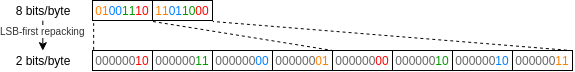
\includegraphics[width=1\textwidth]{img_packets/repacking_lsb.png}
    \caption{Unpacking example for LSB-first, with $X = 2$}
    \label{fig:repacking_lsb}
\end{figure}

\paragraph*{MSB-first repacking}
MSB-first repacking means that the most significant bit of the input byte is read first, and most significant bit of the output byte is filled first.
\begin{figure}[H]
    \centering
    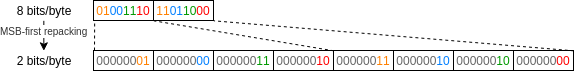
\includegraphics[width=1\textwidth]{img_packets/repacking_msb.png}
    \caption{Unpacking example for MSB-first}
    \label{fig:repacking_msb}
\end{figure}
\newpage
\bibliographystyle{plain}
\begin{thebibliography}{9}
% \bibitem{latexcompanion} 
% Michel Goossens, Frank Mittelbach, and Alexander Samarin. 
% \textit{The \LaTeX\ Companion}. 
% Addison-Wesley, Reading, Massachusetts, 1993.
 
% \bibitem{einstein} 
% Albert Einstein. 
% \textit{Zur Elektrodynamik bewegter K{\"o}rper}. (German) 
% [\textit{On the electrodynamics of moving bodies}]. 
% Annalen der Physik, 322(10):891–921, 1905.
 
% \bibitem{knuthwebsite} 
% Knuth: Computers and Typesetting,
% \\\texttt{http://www-cs-faculty.stanford.edu/\~{}uno/abcde.html
\bibitem{gr_doxygen}
GNU Radio Manual and C++ API Reference
\\\texttt{\small https://gnuradio.org/doc/doxygen/}

\bibitem{packet_header_default_docs} 
gr::digital::packet\_header\_default \quad \textit{ GNU Radio Manual and C++ API Reference }
\\\texttt{\footnotesize https://gnuradio.org/doc/doxygen/classgr\_1\_1digital\_1\_1packet\_\_header\_\_default.html}

\bibitem{corr_est_github_issue} 
{GNU Radio issue \#1207: {Correlation Estimator regression}}\quad \textit{Github}
\\\texttt{\small https://github.com/gnuradio/gnuradio/issues/1207}



\bibitem{gr_pfb} 
gr::filter::pfb\_arb\_resampler\_ccf \quad  \textit{GNU Radio Manual and C++ API Reference}
\\\texttt{\footnotesize https://gnuradio.org/doc/doxygen/classgr\_1\_1filter\_1\_1pfb\_\_arb\_\_resampler\_\_ccf.html}



\bibitem{gr_rrc} 
gr::filter::firdes Class Reference \quad  \textit{GNU Radio Manual and C++ API Reference}
\\\texttt{\footnotesize https://gnuradio.org/doc/doxygen/classgr\_1\_1filter\_1\_1firdes.html}



\bibitem{gr_fec_docs} 
Forward Error Correction\quad \textit{GNU Radio Manual and C++ API Reference}
\\\texttt{\small https://gnuradio.org/doc/doxygen/page\_fec.html}


\bibitem{gr_install} 
Installing GR\quad \textit{GNU Radio Wiki}
\\\texttt{\small https://wiki.gnuradio.org/index.php/InstallingGR}

\bibitem{gr_logging} 
Logging\quad \textit{GNU Radio Manual and C++ API Reference}
\\\texttt{\small https://gnuradio.org/doc/doxygen/page\_logger.html}

\bibitem{gr_development} 
Development\quad \textit{GNU Radio Wiki}
\\\texttt{\small https://wiki.gnuradio.org/index.php/Development}



\end{thebibliography}
\end{document}
